\section{Cohomology}
\subsection{de Rham complex}\index{de Rham!complex}

    \newdef{Exact form}{\index{exact!form}
        A differential form $\omega\in\Omega^k(M)$ such that $\omega=\dr\chi$ for some $\chi\in\Omega^{k-1}(M)$.
    }
    \newdef{Closed form}{\index{closed!form}
        A differential form $\omega\in\Omega^k(M)$ such that $\dr\omega=0$.
    }

    \newdef{de Rham complex}{\label{bundle:closed_exact}
        The sequence
        \begin{gather}
            0\longrightarrow\Omega^0(M)\longrightarrow\Omega^1(M)\longrightarrow\cdots\longrightarrow\Omega^{\dim(M)}(M)\longrightarrow0
        \end{gather}
        together with the sequence of exterior derivatives $\dr_k$ forms a cochain complex by the nilpotency of the exterior derivative. This complex is called the de Rham complex $\Omega^\bullet_\mathrm{dR}(M)$. It encodes the information that every exact form is closed. The converse, however, is not true in general (see \cref{bundle:poincare} below for more information).
    }
    \newdef{de Rham cohomology}{\index{de Rham!cohomology|see{cohomology}}\index{cohomology!de Rham}\label{bundle:de_rham_cohomology}
        Following \cref{homalg:homology}, the $k^{\text{th}}$ de Rham cohomology group on $M$ is defined as the $k^{\text{th}}$ (co)homology group of the de Rham complex:
        \begin{gather}
            H^k_\text{dR}(M) := \frac{\ker(\dr_k)}{\im(\dr_{k-1})}\,.
        \end{gather}
        This quotient space is a vector space. Two elements of the same equivalence class in $H^k_\mathrm{dR}(M)$ are said to be \textbf{cohomologous}.
    }

    \newdef{Integral form}{\label{diff:integral_form}\index{integral!form}
        A closed $k$-form $\omega$ that lies in the image of the inclusion $H^k_\text{dR}(M,\mathbb{Z})\hookrightarrow H^k_\text{dR}(M,\mathbb{R})$. Equivalently, a closed $k$-form is integral if integrating it over any integral $k$-cycle gives an integer.
    }

    \newformula{Cup product}{\index{cup product}\label{bundle:cup_product}
        Let $[\nu]\in H^k_\text{dR}(M)$ and $[\omega]\in H^l_\text{dR}(M)$. The cup product on de Rham cohomology is given by
        \begin{gather}
            [\nu]\smile[\omega] := [\nu\wedge\omega]\,.
        \end{gather}
    }

    The following theorem allows to drop the subscript `$\text{dR}$' when using de Rham cohomology.
    \begin{theorem}[de Rham]\index{de Rham}
        The de Rham cohomology over a smooth manifold is isomorphic to its singular cohomology (\cref{section:singular_homology}).
    \end{theorem}

    \begin{theorem}[Poincar\'e lemma\footnotemark]\index{Poincar\'e!lemma}\label{bundle:poincare}
        \footnotetext{The original theorem states that, on a contractible space (\cref{topology:contractible_space}), every closed form is exact.}
        For every point $p\in M$, there exists a neighbourhood $U\subseteq M$ on which the de Rham cohomology is trivial. More generally, this lemma says that the following isomorphism exists for every smooth manifold $M$:
        \begin{gather}
            H^\bullet(M\times\mathbb{R}^n)\cong H^\bullet(M)\,.
        \end{gather}
        In fact, this can even be further generalized due to the homotopy axiom of de Rham cohomology:
        \begin{gather}
            H^\bullet(E)\cong H^\bullet(M)
        \end{gather}
        for every vector bundle $E$ over $M$.
    \end{theorem}
    \begin{result}
        Every closed form is locally exact, i.e.~if $\dr\omega=0$ at the point $p\in M$, there exist a neighbourhood $U\subseteq M$ of $p$ and a differential form $\lambda$ such that
        \begin{gather}
            \omega=\dr\lambda
        \end{gather}
        at all points of $U$.
    \end{result}

    \newdef{Relative cohomology}{
        Consider the submanifold inclusion $\iota:S\hookrightarrow M$. The relative de Rham complex is defined as follows:
        \begin{gather}
            \Omega^n(M,S) := \Omega^n(M)\oplus\Omega^{n-1}(S)\,,
        \end{gather}
        where the coboundary operator $\dr$ is defined by
        \begin{gather}
            \dr(\omega,\lambda) := (\dr\omega,\iota^*\omega-\dr\lambda)\,.
        \end{gather}
        The relative de Rham cohomology $H^\bullet(M,S)$ is defined as the cohomology of this complex. Classes are represented by closed forms on $M$ that restrict to exact forms on $S$.

        This definition can be generalized to any smooth map $f:M\rightarrow N$ by replacing $\iota^*$ in the coboundary by $f^*$. This cohomology ring is denoted by $H^\bullet(f)$. For all smooth functions $f$, the following long exact sequence exists:
        \begin{gather}
            \cdots\longrightarrow H^k(f)\longrightarrow H^k(M)\longrightarrow H^k(N)\longrightarrow H^{k+1}(f)\longrightarrow\cdots\,.
        \end{gather}
    }

    \newdef{Twisted de Rham complex}{\index{cohomology!twisted}\label{bundle:twisted_de_rham}
        Consider the usual de Rham complex $\Omega^\bullet(M)$ on a smooth manifold $M$. For every degree-3 class $\alpha\in H^3(M)$, one can define the twisted de Rham differential
        \begin{gather}
            \dr_\alpha := \dr + \alpha\wedge\,.
        \end{gather}
        Nilpotency follows from that of $\dr$ and the degree of $\alpha$. The cohomology of this complex is called the ($\alpha$-)twisted de Rham cohomology of $M$.
    }

    The de Rham theorem above can be generalized to the setting of equivariant cohomology (\cref{topology:equivariant_cohomology}).
    \begin{property}[\difficult{Equivariant de Rham theorem}]\index{de Rham}\index{equivariant!cohomology}
        Consider a smooth manifold $M$ with a smooth $G$-action and let $W(\mathfrak{g})$ be the Weil algebra (\cref{lie:weil_algebra}) of $G$. Construct the dgca $\Omega^\bullet(M)\otimes W(\mathfrak{g})$ with differential $\dr_\text{dR}+\dr_\text{W}$. The infinitesimal $G$-action gives a map $\mathfrak{g}\rightarrow\mathfrak{X}(M)$, so Cartan calculus can be extended to all of $\Omega^\bullet(M)\otimes W(\mathfrak{g})$. The \textbf{basic differential forms} are defined as the kernel of the Cartan operators $\iota_\xi,\mathcal{L}_\xi$ for all $\xi\in\mathfrak{g}$. This subcomplex, with the induced differential $\dr_\mathrm{dR}+\dr_\text{W}$, is called the \textbf{Weil model} of equivariant de Rham cohomology.

        If $G$ is compact and connected, the cohomology of the Weil model is isomorphic to the $G$-equivariant cohomology $H_G^\bullet(M)$ from \cref{topology:equivariant_cohomology}.
    \end{property}
    \begin{property}[Cohomological models]
        The intersection of the basic subcomplex with $\Omega^\bullet(M)$ can be identified with the complex of tensorial (basic) differential forms (\cref{bundle:tensorial_form}), i.e.~the pullback $\pi^*\Omega^\bullet(M)\subset\Omega^\bullet(P)$. Moreover, the intersection with the Weil algebra gives a model for the classifying space $BG$ and the Weil algebra gives a model for the total space $EG$.
    \end{property}

\subsection{Integration}\index{co-!chain}

    At this point, a little side note can be given about why the de Rham cohomology groups (\cref{bundle:de_rham_cohomology}) really constitute a cohomology theory. Some concepts from homology are needed that can be found in \cref{section:homology}.

    Let $M$ be a compact manifold. Suppose that one wants to integrate a form over a singular $k$-chain $C\equiv\sum_{i=0}^ka_i\lambda_i$ on $M$. Through integration, one can pair the $k$-form $\omega$ and the singular chain $C$ as if they are dual objects (hence $p$-forms are also called $p$-\textbf{cochains}) to produce a real number:
    \begin{gather}
        \langle\cdot,C\rangle:\Omega^k(M)\rightarrow\mathbb{R}:\omega\mapsto\Int_C\omega := \sum_{i=0}^ka_i\Int_{\Delta_k}\lambda_i^*\omega\,,
    \end{gather}
    where $\lambda_i^*$ pulls $\omega$ back to $\Delta^k$, which is a subset of $\mathbb{R}^k$ as required. Stokes' theorem~\ref{bundle:stokes_theorem} then says that
    \begin{gather}
        \Int_C\dr\omega = \Int_{\partial C}\omega\,.
    \end{gather}
    Using the pairing $\langle\cdot,\cdot\rangle$, this can be rewritten more explicitly as
    \begin{gather}
        \langle\dr\omega,C \rangle = \langle\omega,\partial C\rangle\,.
    \end{gather}
    The operators $\dr$ and $\partial$ can thus be interpreted as formal adjoints. By Stokes theorem, all chains $C$ and cochains $\omega$ belonging to the same equivalence classes $[C]\in H_k(M;\mathbb{R})$ and $[\omega]\in H^k(M;\mathbb{R})$ give rise to the same number $\langle\omega,C\rangle$, so one can see that the singular homology groups and the de Rham cohomology groups on $M$ are well defined dual groups. The name \textit{co}homology is thus well chosen for \cref{bundle:de_rham_cohomology}.

    \begin{remark}[$L^2$-cohomology]\index{cohomology!$L^2$}
        Given a \textit{Riemannian metric} (see \cref{chapter:riemann}), one can define a notion of square-integrable differential forms. The cohomology theory of these forms is called $L^2$-cohomology.
    \end{remark}

\subsection{Cohomology with compact support}\index{cohomology!compact support}\label{section:compact_cohomology}

    Because integration is involved in all statements in this section, it will be assumed that all manifolds and bundles are orientable (unless stated otherwise).

    The following definition characterizes cohomology with compact support directly through its relation to compact sets.
    \newdef{Cohomology with compact support}{\label{bundle:cohomology_compact_support}
        Consider a manifold $M$ (not necessarily orientable). The cohomology with compact support $H^\bullet_c(M)$ is defined as the following direct limit:
        \begin{gather}
            H^\bullet_c(M) := \varinjlim_{\text{compact }K\subseteq M}H^\bullet(M,M\backslash K)\,.
        \end{gather}
    }
    \begin{property}[Relation to reduced cohomology]\label{bundle:reduced_compact_cohomology}
        For a topological space $X$, the inclusion $U\hookrightarrow X$ for any open $U$ induces a long exact sequence in compactly supported cohomology. Performing excision by $V:=X\backslash U$ in the above definition of compact cohomology gives $H^\bullet\bigl(X,X\backslash (K\cup V)\bigr)\cong H^\bullet(U,U\backslash K)$ and thus $H^\bullet_c(X,V)\cong H^\bullet_c(U)$.

        If $X$ is chosen to be the one-point compactification $\widehat{M}$ of $M$ and if $U=M$, the aforementioned long exact sequence implies that
        \begin{gather}
            H^\bullet_c(M)\cong H^\bullet(\widehat{M}, \ast)\cong\widetilde{H}^\bullet(\widehat{M})\,,
        \end{gather}
        where the fact that both $\ast$ and $\widehat{M}$ are compact, which is true for Hausdorff spaces, is used.
    \end{property}

    \begin{theorem}[Poincar\'e duality]\index{Poincar\'e!duality}\label{bundle:poincare_duality}
        Let $M$ be an $m$-dimensional manifold. The pairing $\int:H^k(M)\otimes H^{m-k}_c(M)\rightarrow\mathbb{R}$ induces an isomorphism on cohomology:
        \begin{gather}
            H^k(M)\cong\bigl(H^{m-k}_c(M)\bigr)^*\,.
        \end{gather}
        If $M$ is of finite type (\cref{manifold:good_cover}), the converse also holds:
        \begin{gather}
            H^k_c(M)\cong\bigl(H^{m-k}(M)\bigr)^*\,.
        \end{gather}
    \end{theorem}
    \begin{result}[Poincar\'e lemma for compact cohomology]\index{Poincar\'e!lemma}
        Let $M$ be a (not necessarily orientable) manifold of finite type. For every rank-$n$ vector bundle $E$ over $M$, the following isomorphism exists:
        \begin{gather}
            H^\bullet_c(E)\cong H^{\bullet-n}_c(M)\,.
        \end{gather}
    \end{result}

    \newdef{Poincar\'e dual}{\index{Poincar\'e!dual}
        Let $M$ be an $n$-dimensional manifold and let $i:S\hookrightarrow M$ be a closed $k$-dimensional submanifold. The Poincar\'e dual of $S$ in $M$ is the unique cohomology class $[\eta_S]\in H^{n-k}(M)$ such that
        \begin{gather}
            \Int_Si^*\omega = \Int_M\omega\wedge\eta_S
        \end{gather}
        for all compactly supported $\omega\in H^k_c(M)$. If $S$ is compact in $M$, two Poincar\'e duals exist:
        \begin{itemize}
            \item\textbf{Closed dual}: The Poincar\'e dual obtained by using the fact that $S$ is compact and hence closed in $M$.
            \item\textbf{Compact dual}: Because $S$ is compact, all forms $\omega\in H^k(M)$ (not only the compactly supported ones) can be integrated over $S$ and, assuming $M$ is of finite type, Poincar\'e duality implies that there exists a unique cohomology class with compact support $\eta_S'$ such that
            \begin{gather}
                \Int_Si^*\omega = \Int_M\omega\wedge\eta'_S
            \end{gather}
            for all $\omega\in H^k(M)$.
        \end{itemize}
    }
    \remark{Because the compact Poincar\'e dual induces a pairing on all closed forms $\omega$, which include the compactly supported ones, the compact dual is equal to the closed Poincar\'e dual as a differential form. However, as elements in cohomology these can be quite different.}

    \begin{property}[Localization principle]\index{localization}
        The support of the compact Poincar\'e dual of a compact submanifold $S$ may be shrunk to any neighbourhood of $S$. More generally, the support of the (closed) Poincar\'e dual of a closed submanifold $S$ can be shrunk to any tubular neighbourhood of $S$.
    \end{property}

    \begin{formula}[Transversal intersections]
        The Poincar\'e dual of a transversal intersection is equal to the wedge product of the individual Poincar\'e duals:
        \begin{gather}
            \eta_{S\tpitchfork T} = \eta_S\wedge\eta_T\,.
        \end{gather}
    \end{formula}

    \newdef{Compact vertical cohomology}{\index{cohomology!vertical support}
        Let $\pi:E\rightarrow M$ be a smooth vector bundle over $M$. A differential form $\omega\in\Omega^\bullet(E)$ is said to be an element of $\Omega^\bullet_{\text{cv}}(E)$ if $\supp(\omega)\cap\pi^{-1}(K)$ is compact for every compact subset $K\subseteq M$. The cohomology of this complex is called the \textbf{de Rham cohomology with compact support in the vertical direction}.
    }
    \begin{remark*}
        The above definition implies that $\omega\in\Omega^\bullet_{\text{cv}}(E)$ is compactly supported on the fibre $\pi^{-1}(p)$ for all points $p\in M$. This observation explains the name of the cohomology theory.
    \end{remark*}

    \newdef{Fibre integration}{\index{fibre!intregation}\label{bundle:fibre_integration}
        Differential forms with vertically compact support on a rank-$n$ vector bundle $\pi:E\rightarrow M$ can be divided into two classes:
        \begin{itemize}
            \item\textbf{Type 1}: Those locally of the form $f(x,u)\pi^*\phi\wedge(\dr u_{i_1}\wedge\cdots\wedge \dr u_{i_k})$, where $\phi$ is a form on the base manifold $M$, $f$ has compact support and $k<n$.
            \item\textbf{Type 2}: Those locally of the form $f(x,u)\pi^*\phi\wedge(\dr u_1\wedge\cdots\wedge\dr u_n)$ where $\phi$ is a form on the base manifold $M$ and $f$ has compact support.
        \end{itemize}
        The fibre integration map $\pi_*:\Omega^\bullet_{\text{cv}}(E)\rightarrow\Omega^{\bullet-n}(M)$ is defined as follows. If $\omega$ is of type 1, then $\pi_*\omega:=0$. If $\omega$ is of type 2, then
        \begin{gather}
            \pi_*\omega := \left(\mathlarger{\mathlarger{\idotsint}} f(x,u)\,du_1\cdots du_n\right)\phi\,.
        \end{gather}
    }

    \begin{formula}[Projection formula]\index{projection!formula}
        Consider a rank-$n$ vector bundle $\pi:E\rightarrow M$. For every pair of forms $(\phi,\omega)\in\Omega^\bullet(M)\times\Omega^\bullet_{\text{cv}}(E)$, the following formula holds:
        \begin{gather}
            \pi_*(\pi^*\phi\wedge\omega) = \phi\wedge\pi_*\omega\,.
        \end{gather}
        Furthermore, if $\phi\in\Omega^k_c(M)$ and $\omega\in\Omega^{m+n-k}_{\text{cv}}(E)$,
        \begin{gather}
            \Int_E\pi^*\phi\wedge\omega = \Int_M\phi\wedge\pi_*\omega\,.
        \end{gather}
    \end{formula}

    \begin{theorem}[Thom isomorphism]\index{Thom!isomorphism}\label{bundle:thom_isomorphism}
        For every rank-$n$ vector bundle $\pi:E\rightarrow M$, where $M$ is (not necessarily orientable and) of finite type, fibre integration gives the following isomorphisms:
        \begin{gather}
            \pi_*:H^\bullet_{\text{cv}}(E)\cong H^{\bullet-n}(M):\mathcal{T}\,.
        \end{gather}
    \end{theorem}
    \begin{result}[Poincar\'e lemma for vertically compact cohomology]\index{Poincar\'e!lemma}
        \begin{gather}
            H^\bullet_{\text{cv}}(M\times\mathbb{R}^n)\cong H^{\bullet-n}(M)
        \end{gather}
    \end{result}

    \begin{formula}[Thom isomorphism]\index{Thom!class}\index{Thom!isomorphism}
        Define the \textbf{Thom class} of $M$ as $\Phi:=\mathcal{T}(1)\in H^0(M)$. Because $\mathcal{T}$ and $\pi_*$ are mutual inverses and, hence, $\pi_*\Phi=1$, the projection formula implies that
        \begin{gather}
            \mathcal{T}(\omega) = \pi^*\omega\wedge\Phi\,.
        \end{gather}
    \end{formula}

    \begin{property}[Orientation class]\index{orientation!class}
        The Thom class $\Phi$ restricts to a generator of the cohomology of the typical fibre $V$:
        \begin{gather}
            H^n_c(V)\cong\widetilde{H}^n(S^n)\cong H^n(S^n)\,.
        \end{gather}
        For compact orientable manifolds, such a generator gives rise to a generator of the homology group $H_n$, i.e.~it gives rise to an orientation class (\cref{bundle:orientation_class}).
    \end{property}
    \begin{property}[Poincar\'e dual]\index{Poincar\'e!dual}
        The Poincar\'e dual of a closed submanifold is equal to the Thom class of its normal bundle.
    \end{property}

    The construction of the Thom isomorphism involves some technicalities. For example, throughout the literature, the Thom isomorphism is stated in various forms using compactly supported cohomology, relative cohomology or reduced cohomology. The various approaches are related as follows.
    \newdef{Thom space}{\index{Thom!space}\index{sphere!bundle}
        Let $E\rightarrow M$ be a vector bundle. For every fibre in $E$, one can construct its one-point compactification (\cref{topology:alexandrov_compactification}) and, by gluing these together, the \textbf{sphere bundle} $\mathrm{Sph}(E)$ is obtained. The quotient space $\mathrm{Sph}(E)/B$, where all the adjoined points are identified, is called the Thom space $\mathrm{Th}(E)$.

        By equipping $E$ with a \textit{metric} (see \cref{chapter:riemann}), one can give an alternative definition. Let $V$ be the typical fibre of $E$. A new bundle, the unit sphere bundle $S(E)$, where the typical fibre is the unit sphere $S(V) := \{v\in V\mid\|v\| = 1\}$, can now be constructed. (It should be noted that this new bundle is not a vector bundle since the unit sphere is not a vector space.) A similar construction leads to the unit disk bundle $D(E)$, where the typical fibre is the unit disk $D(V) := \{v\in V\mid\|v\|\leq1\}$. The Thom space $\mathrm{Th}(E)$ can be shown to be isomorphic to the quotient space $D(E)/S(E)$.
    }
    \begin{property}
        If the base manifold $M$ is compact, the Thom space is obtained as the one-point compactification of the total space $E$.
    \end{property}

    \begin{property}[Different forms of Thom isomorphism]
        Let $E\rightarrow M$ be a vector bundle and denote the complement of the zero section by $E_0$ as in \cref{bundle:zero_section}. Homotopy invariance implies that
        \begin{gather}
            H^\bullet\bigl(D(E),S(E)\bigr)\cong H^\bullet(E,E_0)\,.
        \end{gather}
        Then, using \cref{bundle:ndr_submanifold} together with the dual of \cref{topology:ndr_pair_homology}, one can show that the reduced cohomology of the Thom space $\mathrm{Th}(E)$ is isomorphic to the relative cohomology of the pair $(E,E_0)$:
        \begin{gather}
            \widetilde{H}^\bullet\bigl(\mathrm{Th}(E)\bigr)\cong H^\bullet(E,E_0)\,.
        \end{gather}
        To relate this to vertically compact cohomology, \cref{bundle:reduced_compact_cohomology} can be adapted. Compact support gave rise to the (reduced) cohomology of the compactified space. By analogy, vertically compact support corresponds to compactifications of the fibres, which is exactly how the Thom space is constructed.

        The above arguments finally lead to the following triangle of isomorphisms:
        \begin{gather}
            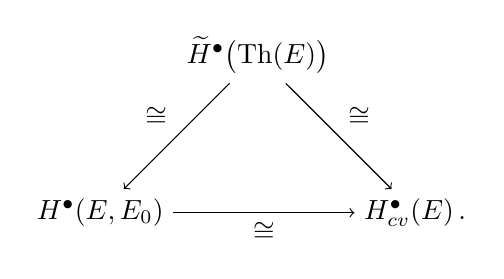
\begin{tikzpicture}[baseline=(current bounding box.east)]
                \node (TH) at (0, 0) {$\widetilde{H}^\bullet\bigl(\mathrm{Th}(E)\bigr)$};
                \node (R) at (-2, -2) {$H^\bullet(E,E_0)$};
                \node (CV) at (2, -2) {$H^\bullet_{\text{cv}}(E)\,.$};
                \draw[->] (TH) -- node[above left]{$\cong$} (R);
                \draw[->] (TH) -- node[above right]{$\cong$} (CV);
                \draw[->] (R) -- node[below]{$\cong$} (CV);
            \end{tikzpicture}
        \end{gather}
    \end{property}

    \newdef{\difficult{Thom spectrum}}{\index{spectrum!Thom}
        Let $E\rightarrow M$ be a vector bundle. The Thom spectrum of $E$ is defined as the suspension spectrum of its Thom space:
        \begin{gather}
            (\Sigma^\infty\mathrm{Th}(E))_n\cong\mathrm{Th}(\mathbb{R}^n\oplus E)\,,
        \end{gather}
        where $\mathrm{Th}(\mathbb{R}^n\oplus E)\cong\Sigma^n\mathrm{Th}(E)$ was used.

        Now, consider the sequence $\seq{\xi}$ of \textit{universal vector bundles}. For every $\xi_n$, define the $n^{\text{th}}$ component space as follows:
        \begin{gather}
            MO_n := \mathrm{Th}(\xi_n)\,.
        \end{gather}
        The Whitney sum $\xi_n\oplus\mathbb{R}$ can be obtained as a pullback of $\xi_{n+1}$. This map induces a morphism $\Sigma MO_n\rightarrow MO_{n+1}$, which gives the $n^{\text{th}}$ structure map of `the' Thom spectrum $MO$.\footnote{Note that the Thom spectrum as defined here is not an $\Omega$-spectrum (\cref{topology:spectrum}), it is merely a sequential spectrum (prespectrum).}
    }

    \newdef{Euler class}{\index{Euler!class}
        Consider a vector bundle $E\rightarrow M$ together with its Thom class $\Phi$. The Euler class $e(E)$ is defined as the pullback $s_0^*\Phi$ of the Thom class along the zero section of $E$.
    }
    \begin{property}
        If the orientation of $E$ is reversed, the Euler class changes sign.
    \end{property}
    The following property distinguishes the Euler class among all characteristic classes of $E$.
    \begin{property}[Normalization]
        If the vector bundle admits a nowhere-vanishing section, its Euler class vanishes.
    \end{property}

\subsection{\v{C}ech--de Rham complex}\label{section:cech_de_rham}

    \begin{theorem}[Mayer--Vietoris sequence]\index{Mayer--Vietoris!sequence}
        Consider a smooth manifold $M$ with an open covering $U\cup V$. The cohomology of $U,V$ is related to that of $M$ by the following short exact sequence:
        \begin{gather}
            0\longrightarrow H^\bullet(M)\overset{\iota_U\oplus\iota_V}{\longrightarrow} H^\bullet(U)\oplus H^\bullet(V)\overset{\pi_2-\pi_1}{\longrightarrow} H^\bullet(U\cap V)\longrightarrow 0\,.
        \end{gather}
    \end{theorem}

    \newdef{\v{C}ech--de Rham complex}{
        The \v{C}ech complex (\cref{sheaf:cech}) associated to the constant sheaf $\flat\mathbb{R}$, i.e.~the sheaf of locally constant functions.
    }

    The Mayer--Vietoris sequence can be generalized to a statement about the \v{C}ech-de Rham complex.
    \begin{property}[Mayer--Vietoris sequence]
        The horizontal complex
        \begin{gather}
            0\longrightarrow\Omega^\bullet(M)\longrightarrow\prod_{i_0}\Omega^\bullet(U_{i_0})\longrightarrow\prod_{i_0,i_1}\Omega^\bullet(U_{i_0i_1})\longrightarrow\cdots
        \end{gather}
        is acyclic, i.e.~the $\delta$-cohomology of the \v{C}ech--de Rham complex vanishes.
    \end{property}

    An important corollary is that one can compute the (de Rham) cohomology of $M$ using the above double complex.
    \begin{property}
        The restriction map $\Omega^\bullet(M)\rightarrow C^\bullet(\mathcal{U};\Omega^\bullet)$ induces an isomorphism in cohomology.
    \end{property}
    One can also augment the \v{C}ech--de Rham complex in the other direction by the kernel of the de Rham differential in degree 1. These are the locally constant functions on the intersections $U_{i_0\ldots i_p}$. The cohomology of this augmenting sequence $C^\bullet(\mathcal{U};\flat\mathbb{R})$ is called the \textbf{\v{C}ech cohomology} of $M$.\index{Cech!cohomology} By the same reason as for why the Mayer--Vietoris sequence implied the above theorem, the following theorem is obtained.
    \begin{theorem}[\v{C}ech $=$ de Rham]
        For a smooth manifold $M$, admitting a good cover $\mathcal{U}$, the \v{C}ech cohomology of $\mathcal{U}$ is isomorphic to the de Rham cohomology of $M$:
        \begin{gather}
            H^\bullet(M)\cong\check{H}^\bullet(\mathcal{U};\flat\mathbb{R})\,.
        \end{gather}
        By noting that good covers are \textit{cofinal} in the set of open covers, one can pass to the full \v{C}ech cohomology:
        \begin{gather}
            H^\bullet(M)\cong\check{H}^\bullet(M;\flat\mathbb{R})\,.
        \end{gather}
    \end{theorem}
    \begin{result}
        All compact manifolds admit a finite good cover and, hence, have finite-dimensional de Rham cohomology.
    \end{result}

    \begin{property}[Exponential sequence]
        Consider the following exact sequence of topological groups:
        \begin{gather}
            0\longrightarrow\mathbb{Z}\overset{2\pi}{\longrightarrow}\mathbb{C}\overset{\exp}{\longrightarrow}\mathrm{U}(1)\longrightarrow0\,.
        \end{gather}
        Let $(M,\mathcal{O}_M)$ be a \textit{complex manifold} (see \cref{chapter:complex_geometry}) or a smooth manifold and restrict the above sequence to the real numbers. The exact sequence induces an exact sequence of structure sheaves:
        \begin{gather}
            0\longrightarrow\flat\mathbb{Z}\longrightarrow\mathcal{O}_M\longrightarrow\mathcal{O}_M^\times\longrightarrow0\,.
        \end{gather}
        This, in turn, induces a long exact sequence in cohomology and, by \cref{sheaf:example_soft} (if $M$ is paracompact), the connecting homomorphism leads to an isomorphism:
        \begin{gather}
            \label{bundle:U1_cohomology_isomorphism}
            H^{\bullet+1}(M;\mathbb{Z})\cong\check{H}^\bullet\bigl(M;\mathrm{U}(1)\bigr)\,.
        \end{gather}
        Note that the cohomology on the right-hand side is not singular cohomology. Singular $\mathrm{U}(1)$-valued cohomology could also be related to integral cohomology through the \textit{universal coefficient theorem}, but extra terms involving Ext-functors would appear.
    \end{property}

\subsection{Nonorientable manifolds}

    This section gives a differential-geometric incarnation of \cref{section:local_coefficients} on local coefficients.

    \newdef{Twisted cohomology}{\index{cohomology!twisted}
        Let $E\rightarrow M$ be a flat vector bundle over $M$. By \cref{bundle:twisted_differential}, the algebra $\Omega^\bullet(M)\otimes E$ can be given the structure of a differential graded algebra (\cref{homalg:dg_algebra}) and, hence, gives rise to a cohomology theory $H^\bullet(M;E)$. This is called the $E$-twisted de Rham cohomology of $M$.
    }
    \begin{remark}
        According to the remark following \cref{bundle:twisted_differential}, attention should be payed to which trivialization was used in the construction of $H^\bullet(M;E)$. However, it can be shown that two trivializations give rise to the same $E$-twisted cohomology if they admit a common refinement for which the induced sections differ by a locally constant matrix in $\GL(n,\mathbb{R})$.
    \end{remark}

    If one takes $E=o(M)$ to be the orientation line bundle over $M$, the (honest) densities of \cref{bundle:honest_density} are obtained. The cohomology of this complex is simply called the \textbf{twisted de Rham cohomology}.
    \begin{property}[Isomorphism]
        The twisted cohomologies defined by two trivializations induced from atlases on $M$ are isomorphic.\footnote{Although one almost always works with a natural trivialization, i.e.~the open subsets of $M$ are obtained from charts on $M$, this is technically not necessary. For more `exotic' cases, the isomorphisms not always exist.}
    \end{property}
    \begin{property}[Trivial twisting]
        If $M$ is orientable, its twisted cohomology is isomorphic to its ordinary (de Rham) cohomology. More generally, the $E$-twisted de Rham cohomology is isomorphic to the ordinary de Rham cohomology whenever $E$ is trivial.
    \end{property}

    Poincar\'e duality (\cref{bundle:poincare_duality}) can be generalized almost verbatim to the twisted case.
    \begin{theorem}[Poincar\'e duality]\index{Poincar\'e!duality}
        Integration of densities induces the following isomorphism:
        \begin{gather}
            H^k(M)\cong\left(H^{m-k}_c\bigl(M;o(M)\bigr)\right)^*\,.
        \end{gather}
        If $M$ is of finite type, the converse also holds:
        \begin{gather}
            H^k_c(M)\cong\left(H^{m-k}\bigl(M;o(M)\bigr)\right)^*\,.
        \end{gather}
    \end{theorem}
    The Thom isomorphism also holds for nonorientable bundles.
    \begin{theorem}[Thom isomorphism]\index{Thom!isomorphism}
        Let $E\rightarrow M$ be a rank-$n$ vector bundle. Fibre integration gives the following isomorphism:
        \begin{gather}
            H^{\bullet+n}_{\text{cv}}(E)\cong H^\bullet\bigl(M;o(E)\bigr)\,.
        \end{gather}
    \end{theorem}

\subsection{\difficult{Generalized cohomology}}

    In this section, some statements from singular/de Rham cohomology on vector bundles are generalized to statements about the generalized (Eilenberg--Steenrod) cohomology theories from \cref{section:eilenberg_steenrod}. In the remainder of this section, $E^\bullet$ will denote a multiplicative generalized cohomology theory.\footnote{`Multiplicative' indicates that there exists a cup product such that every group $E^\bullet(M)$ becomes a graded ring.}

    \newdef{Orientation}{\index{orientation}\index{Thom!class}
        Consider a rank-$n$ vector bundle with typical fibre $V$. An $E$-orientation or $E$-\textbf{Thom class} is a cohomology class $u\in\widetilde{E}^n(\mathrm{Th}(V))$ that restricts to a generator on every fibre of $V$.
    }

    \todo{COMPLETE}